\documentclass{article}
\usepackage[utf8]{inputenc}

\title{MATH3160 — Portfolio 4.4, 5.2-5.4}
\author{Mike Medved}
\date{October 31st, 2022}

\usepackage{color}
\usepackage{amsthm}
\usepackage{amssymb} 
\usepackage{amsmath}
\usepackage[margin=1in]{geometry} 
\usepackage{listings}
\usepackage[dvipsnames]{xcolor}
\usepackage{tikz}

\newtheorem*{thm}{Theorem}

\begin{document}

\maketitle

\section{Deliverables}

\subsection{Continuous vs Discrete Tools}

\begin{table}[!htb]
    \centering
    \begin{tabular}{|l|l|l|}
    \hline
                                                                                 & \textbf{Discrete}                                                                         & \textbf{Continuous}                                                                          \\ \hline
    \textbf{Image}                                                                & Finite / Countable                                                                        & Interval (Infinite + Uncountable)                                                            \\ \hline
    \textbf{\begin{tabular}[c]{@{}l@{}}Probabilities of Interest\end{tabular}} & $P(X = a)$, $a \in \text{Im X}$                                                           & \begin{tabular}[c]{@{}l@{}}$P(X \in I)$, where $I$ is an interval on $\mathbb{R}$\end{tabular} \\ \hline
    \textbf{Density}                                                                   & $\displaystyle\sum_{x \in \text{Im X}} f(x) = 1$                                                                 & $\displaystyle\int_{\mathbb{R}} f(x) dx = 1$                                                                 \\ \hline
    \textbf{Distribution}                                                                   & \begin{tabular}[c]{@{}l@{}}$F(X) = \displaystyle\sum_{t \leq x} f(t)$, $t \in \text{Im X}$\end{tabular} & $F(X) = \displaystyle\int_{-\infty}^{-x} f(t) dt$                                                      \\ \hline
    \textbf{Expectation}                                                            & $\displaystyle\sum_{x \in \text{Im X}} x*f(x)$                                                                        & $\displaystyle\int_{\mathbb{R}} x*f(x)dx$                                                                  \\ \hline
    \textbf{Moment Generating Function}                                                         & $\displaystyle\sum_{x \in \text{Im X}} g(x)*f(x)$                                             & $\displaystyle\int_{\mathbb{R}} g(x)*f(x) dx$                                           \\ \hline
    \textbf{Variance}                                                              & $E\left[X^2\right] - \left(E\left[X\right]\right)^2$                                 & $E\left[X^2\right] - \left(E\left[X\right]\right)^2$                                    \\ \hline
    \end{tabular}
\end{table}

\subsection{Uniform Random Variable Example}

\begin{center}
    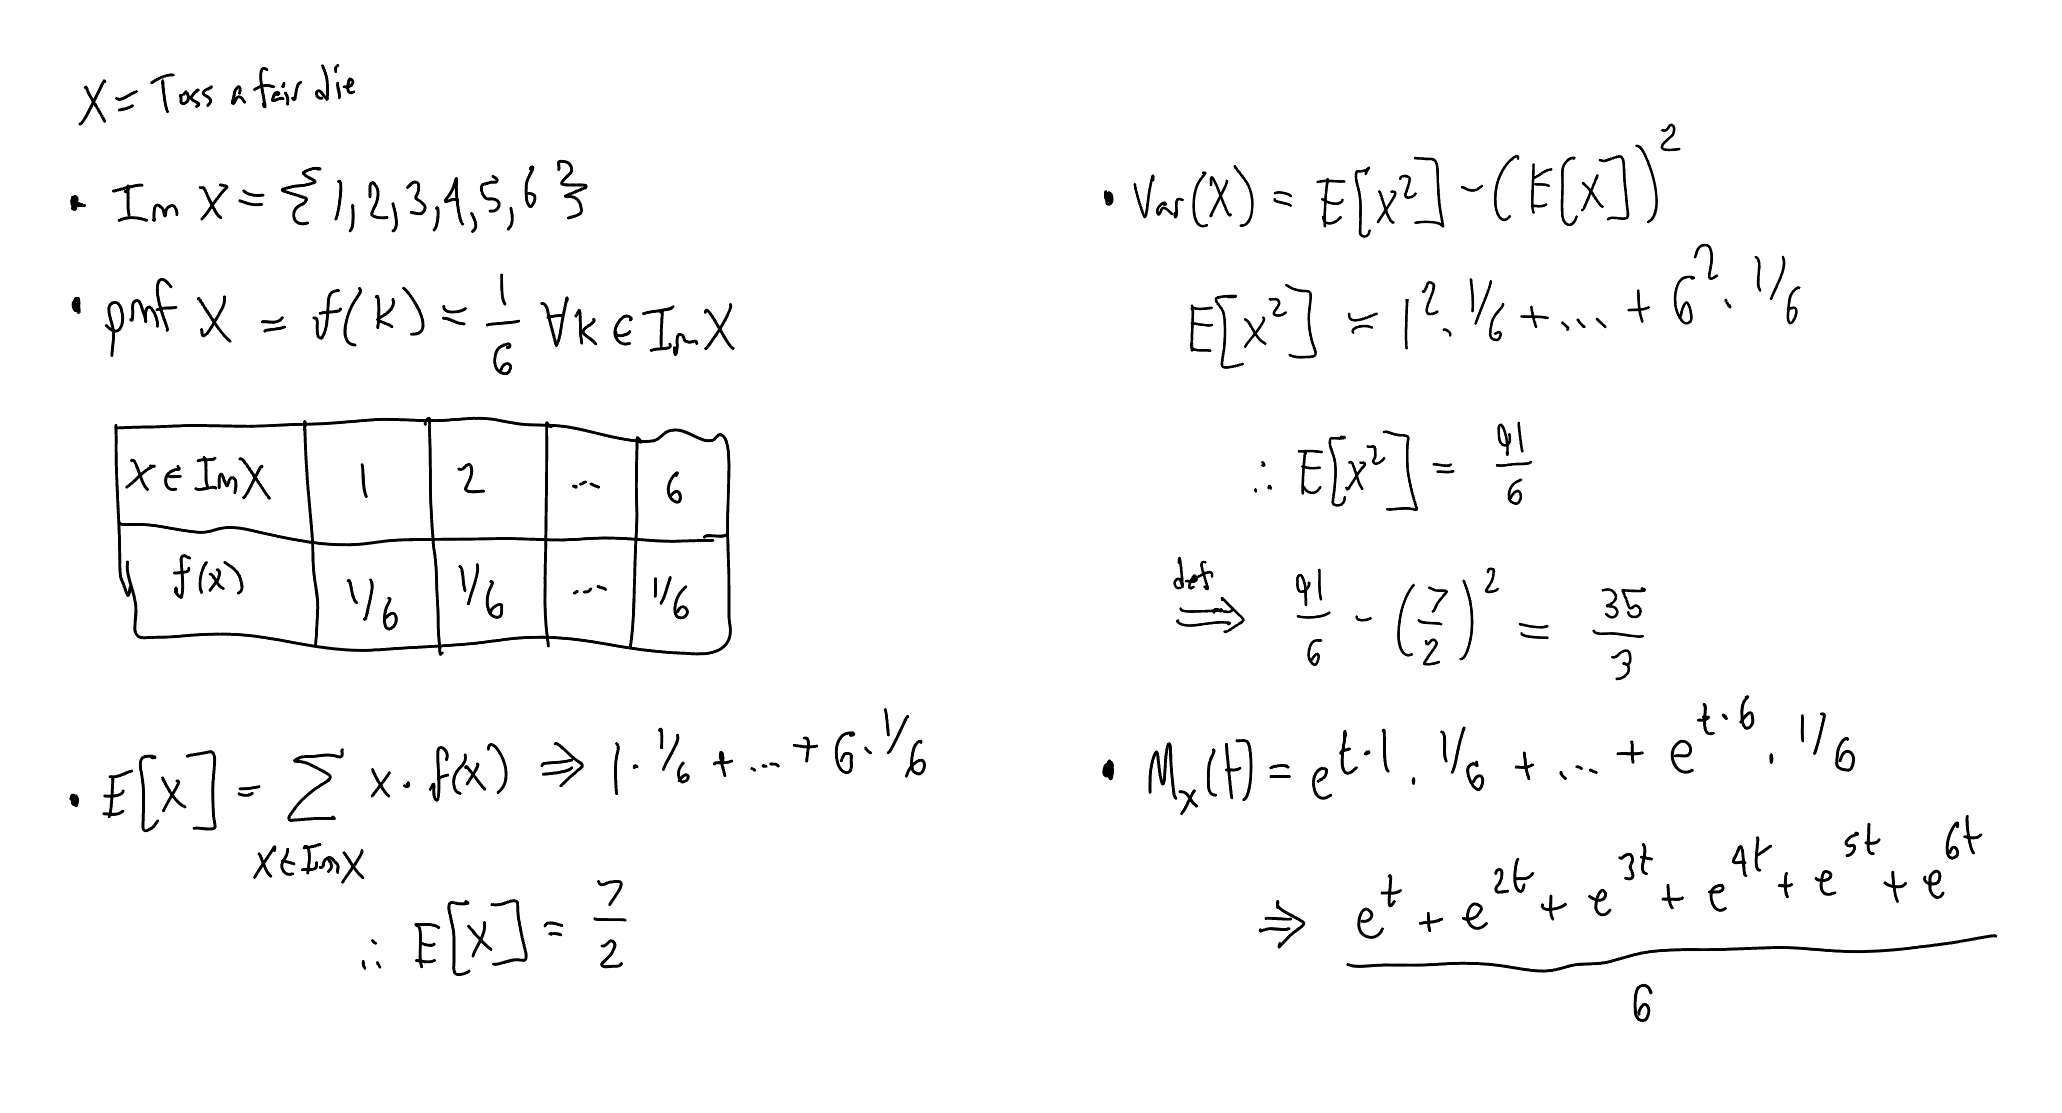
\includegraphics[height=3in]{q2.jpeg}
\end{center}

\subsection{Bernoulli Random Variable Example}

\begin{center}
    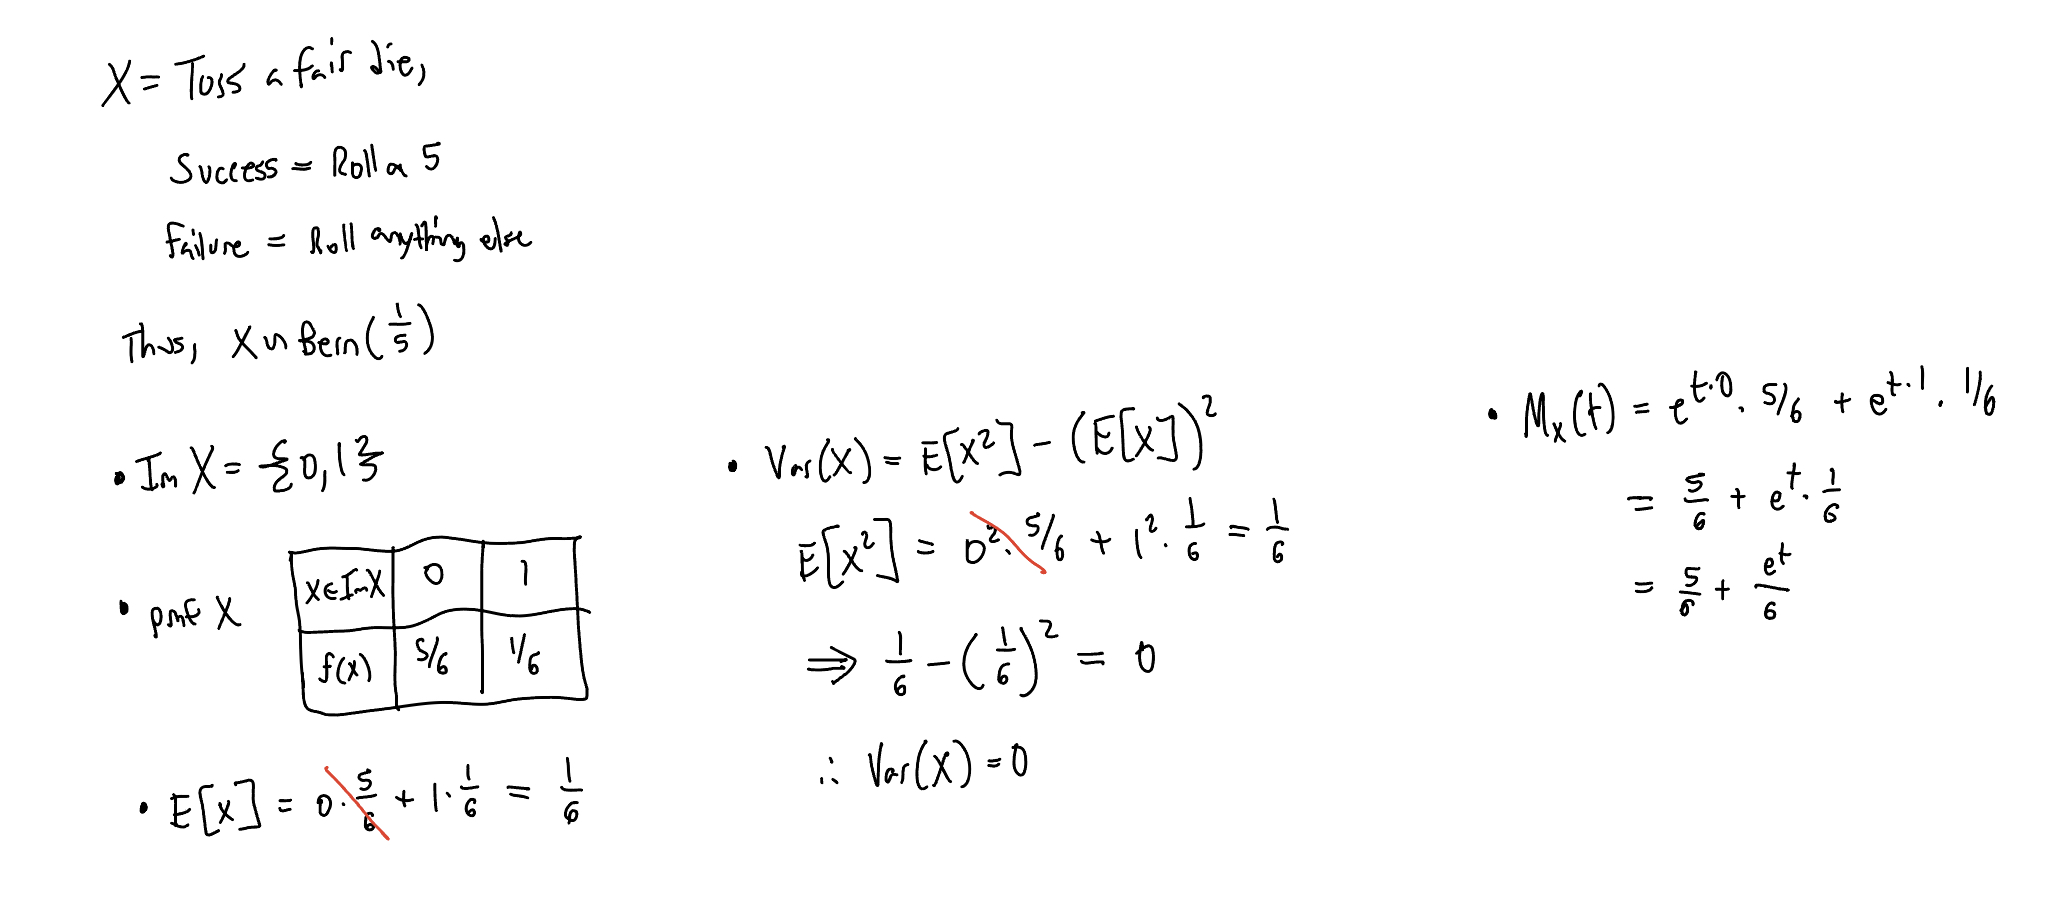
\includegraphics[height=3in]{q3.jpeg}
\end{center}

\subsection{Binomial Random Variables}

A binomial random variable of parameters $n, p$ is the number of successes in $n$ independent \textit{Bern(p)} trials. This is denoted as $X \sim \text{Bin}(n, p)$, and is actually one of the representations of the Bernoulli random variable, as such: $\text{Bern}(p) \Longleftrightarrow \text{Bin}(1, p)$.

$\hfill \break$
Further, as the Bernoulli random variable is a special case of the binomial random variable, we can use the same formula for the expectation and variance of the binomial random variable as we did for the Bernoulli random variable.

$\hfill \break$
In this way, we can express binomial random variables as their Bernoulli components:

$$
X = \sum_{i=1}^n X_i
$$

$\hfill \break$
where $X_i \sim \text{Bern}(p)$. In this way, we can use the same formula for the expectation and variance of the binomial random variable as we did for the Bernoulli random variable.

\subsubsection{Example of computation}

\begin{center}
    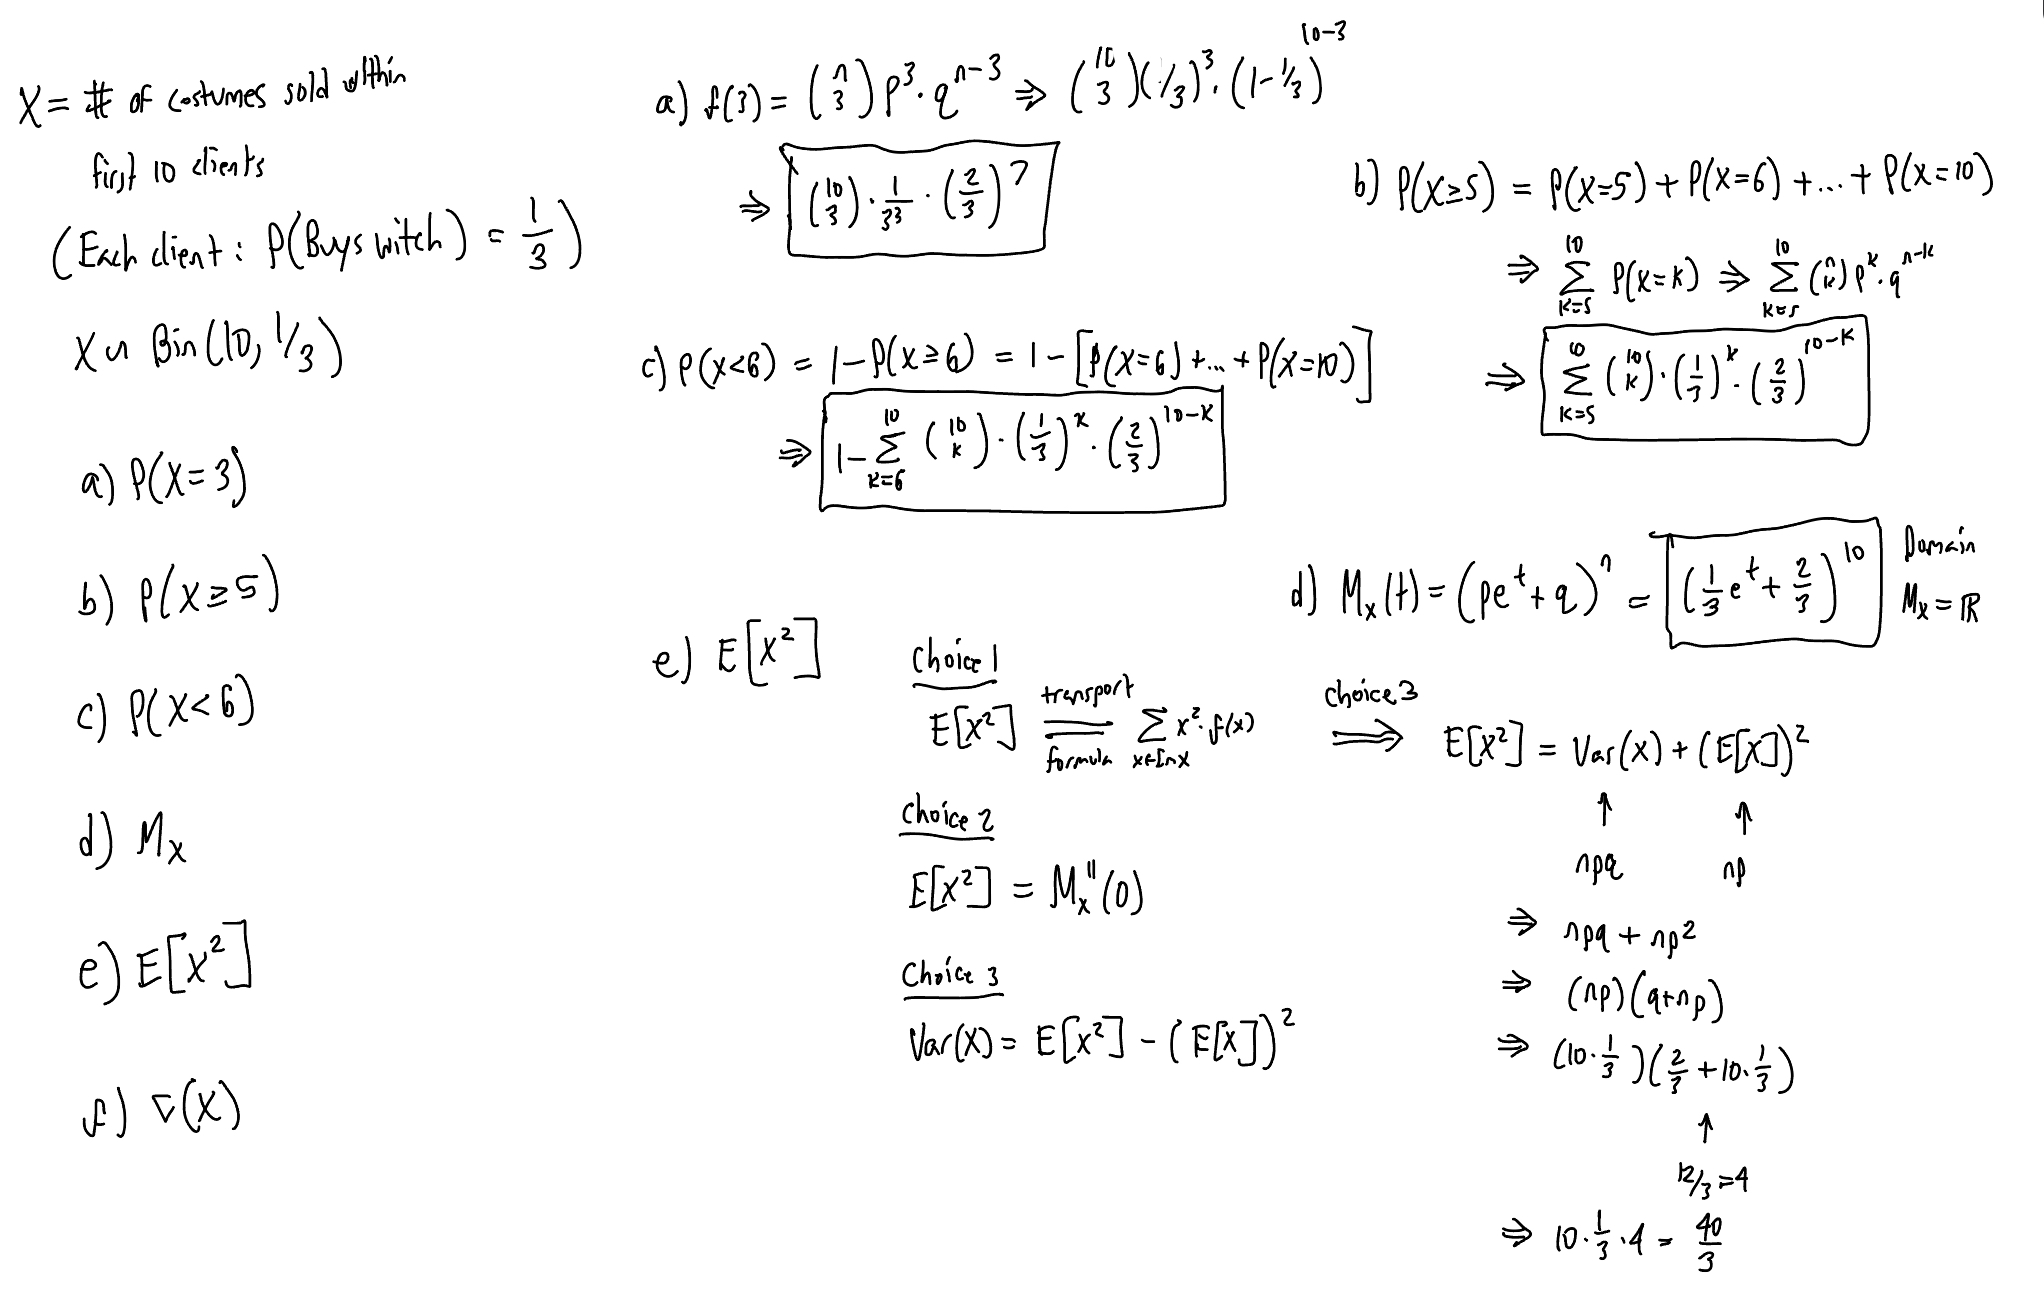
\includegraphics[height=4in]{q4.jpeg}
\end{center}

\end{document}